\chapter{Background and Literature Review}
\section{ The National Electricity Market }
The NEM began to operate on December 1998, as part of the Australian power industry. The NEM is defined as restructured electricity industry with a gross pool market\footnote{A gross pool market refers to an electricity market where all generators are required to sell \textit{all} the energy there produce, in the case of the NEM this is done via the Australian Energy Market Operator (AEMO). A gross pool market differs from a net pool market where generators only sell energy that they have not already sold through bilateral contracts.}. The NEM is multi-regional with intra-regional loss factors connecting the eastern and southern states and territories of: Queensland (QLD); New South Wales (NSW); Victoria (VIC); South Australia (SA); Tasmania (TAS) and the Australian Capital Territory (ACT). Within the NEM, the COAG Energy Council is the key decision maker with policy and governance responsibility. The Australian Energy Market Commission (AEMC) develops the rules by which the market must operate. The Australian Energy Market Operator (AEMO) handles the day-to-day operations of the electricity and gas markets, with The Australian Energy Regulator (AER) enforcing the rules and making judgement on the regulatory proposals of monopoly network operators \parencite{EnergyGov}. 
\subsection{ Operation of the Spot Market }
To ensure the output from all NEM generators are scheduled to instantaneously match real-time consumer demand, AEMO dispatches all generators through a centrally coordinated process. This process involves generators submitting price/quantity pairs of electricity bids that they are willing to generate to AEMO. AEMO’s central dispatch engine (NEMDE) orders the generators’ offers in a merit-order fashion to determine lowest cost mix of generators dispatched at a given time. In delivering electricity, AEMO dispatches electricity every five minutes, so generators are required to bid to supply electricity in five minute blocks. For the purposes of settlement, the price is then averaged out over 30 minutes. The AEMC has recently completed assessment of a proposal to change the time interval for settlement in the wholesale electricity market from 30 minutes to five minutes. This change is to be introduced with effect from 1 July 2021 \parencite{5minSettle}. The Market Price Cap, which is the maximum spot price, is \$14,500/MWh. This is the maximum price at which generators can bid into the market. The Market Floor Price, which is the lowest spot price, is -\$1,000/MWh. This creates the possibility of large spreads in electricity prices, as well as momentary price spikes.
\subsection{ Operation of the Ancillary Service Market }
AEMO uses ancillary services to manage security and reliability within the NEM, by controlling frequency and voltage levels. Ancillary services are grouped into the following categories:
\begin{enumerate}
    \item Frequency Control Ancillary Services (FCAS)
    \item Network Support \& Control Ancillary Services (NSCAS)
    \item System Restart Ancillary Services (SRAS)
\end{enumerate}
\subsubsection{Frequency Control Ancillary Services (FCAS)} \label{fcas}
The NEM Mainland Frequency Operating Standard sets the grid frequency to remain between 49.85 to 50.15 Hertz (Hz) for 99 per cent of normal operation \parencite{FrequencyReq}. FCAS can be broken down into two markets, Contingency and Regulation. FCAS Contingency is used infrequently, it involves correcting deviations in load and generation following a major, unexpected event, such as a generator or transmission line disconnecting \parencite{Boyle}.  In contrast, FCAS Regulation acts to continuously ensure load balances with generation and correct any minor frequency deviations.
\newline
\newline
Unlike regulation, contingency services must always be enabled despite only being utilised occasionally.. Following a contingency event AEMO has five minutes to return the frequency to the normal operating band \parencite{FrequencyReq}. There are six markets within FCAS Contingency, consisting of a Raise and Lower market for the three response intervals. These three intervals are fast at six seconds, Slow at one minute and delayed at five minutes. There are two markets within FCAS Regulation, these are Regulation Raise, correcting any frequency drops and Regulation Lower, which corrects any frequency rises. Generators and loads submit bids to participate in the eight FCAS markets every five minutes, via AEMO’s Market Management Systems (MMS). AEMO then co-optimises both the wholesale and FCAS markets to determine dispatch and payments. Automated Generation Control (AGC) is the mechanism through which generators provide frequency regulation services. AEMO continuously monitors frequency via the AGC system, sending signals to generators when there are any minor frequency deviations, which need to be corrected.
\subsection{ Pre-dispatch Forecast Process }
Within the NEM, a pre-dispatch process is performed by AEMO to ensure that market participants have sufficient pricing information to make informed and timely business decisions. In turn, this information provides the market with the information it needs to provide security of supply.  AEMO publishes somewhat limited information during pre-dispatch, however in evaluating battery storage this is vital to ensuring appropriate state of charge for future energy arbitrage opportunities. AEMO processes 3 different pre-dispatch methods to forecast price, 5 minute, 30 minute and predispatch sensitivities.
\subsubsection{P5 Region Solution}
\label{sec:background_p5}
The 5-minute pre-dispatch cycle runs every 5-minutes to produce a dispatch and pricing schedule to a 5-minute resolution covering the next hour, for a total of twelve periods. It is key to note these prices represent forecasts for 5 minute dispatch prices rather than trading prices. Figure \ref{fig:p5_process_1} shows predicted dispatch price via the P5 Region Solution within the trading interval of 12:30:00pm, on the 1st of January, 2018, in South Australia. 
\begin{figure}[H]
\centering
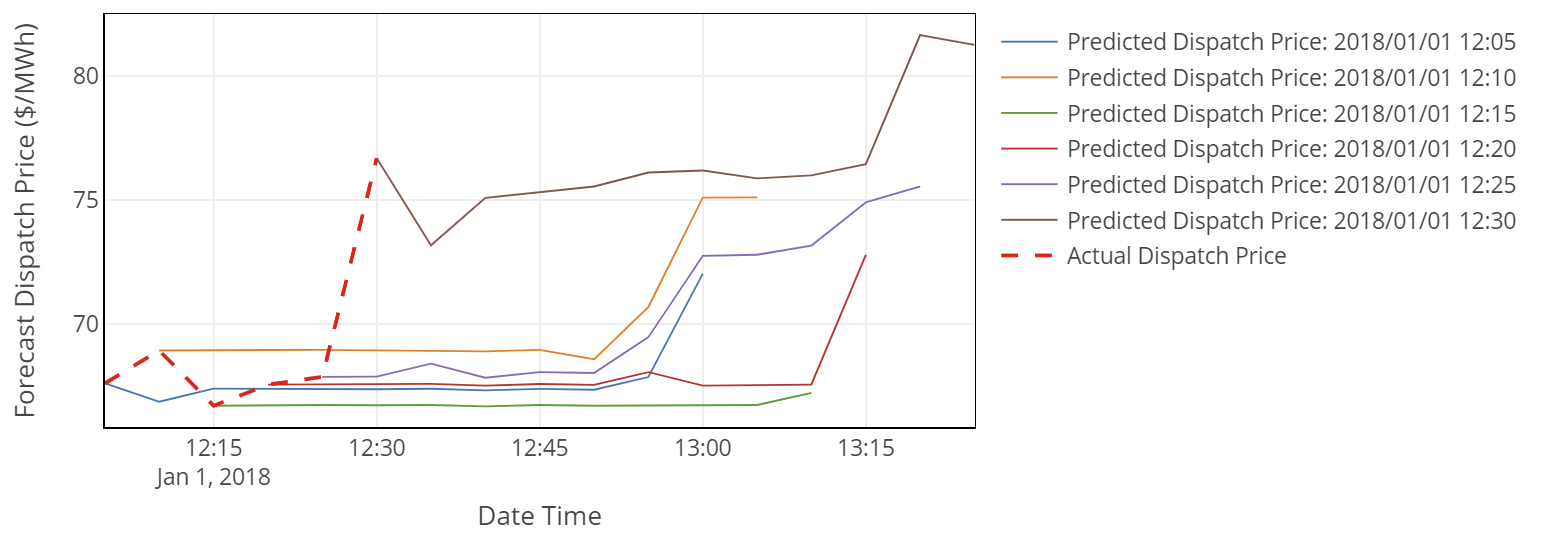
\includegraphics[width=0.8\textwidth]{Pictures/Chapter2/P5_Process.png}
\caption{P5 Predispatch Process - South Australia, Trading Interval 01/01/2018 12:30:00 PM}
\label{fig:p5_process_1}
\end{figure}
As seen in Figure \ref{fig:p5_process_1}, the P5 Region solution runs each 5 minutes and accuracy converges as forecast period approaches the dispatch interval. Although the forecast may not appear very accurate, Figure \ref{fig:p5_process_2} shows the P5 Price forecast elapsed for a full 24 hrs, clearly showing price follows the trend set by the forecast. 
\begin{figure}[H]
\centering
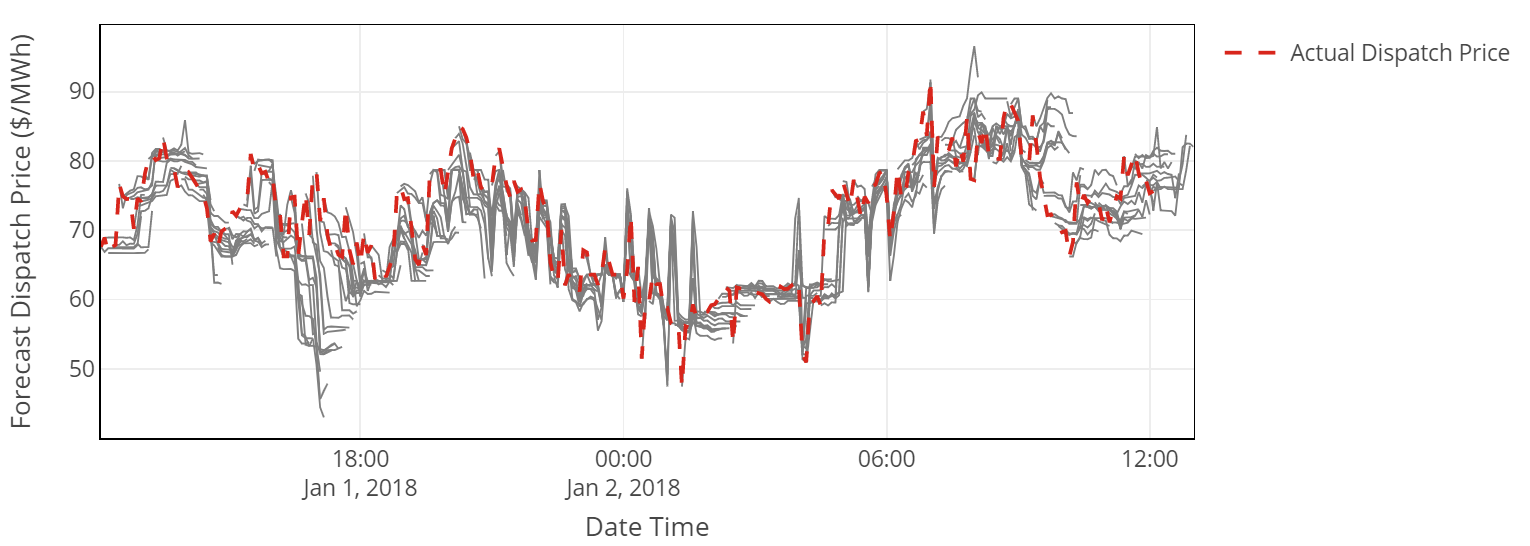
\includegraphics[width=1\textwidth]{Pictures/Chapter2/P5_Process_2.png}
\caption{P5 Pre-dispatch Process - South Australia, 01/01/2018 - 02/01/2018}
\label{fig:p5_process_2}
\end{figure}
To date, no peer-reviewed academic analysis has been performed on the accuracy of the P5 Price forecast. The fundamental justification is most likely the shear size of the data set \textit{(For each year there are over 6 million rows of data for the 5 NEM jurisdictions)}. However, \parencite{AEMCMarch2017} provides insight into the magnitude of P5 Price forecast error by NEM region for the period 1 September 2015 to 8 March 2017, as shown in Figure \ref{fig:p5_aemc}. 
\begin{figure}[H]
\centering
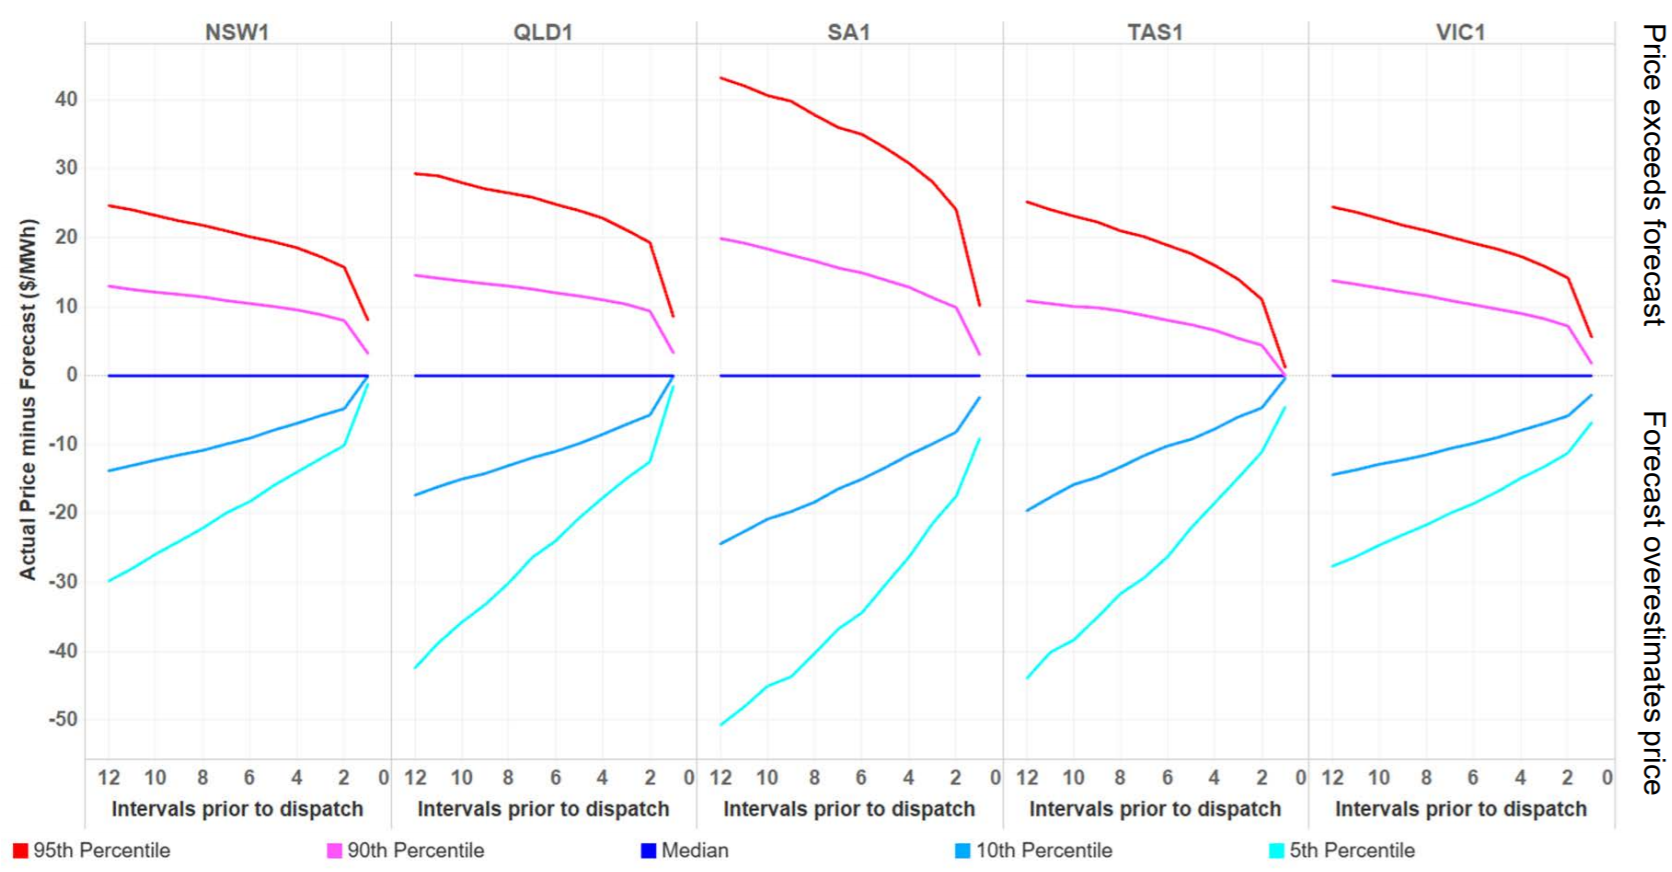
\includegraphics[width=1\textwidth]{Pictures/Chapter2/AEMC_P5_Error.PNG}
\caption{AEMC 2017: Magnitude of Forecast Error Varies by Region.}
\label{fig:p5_aemc}
\end{figure}
\parencite{AEMCMarch2017} highlights 3 key elements regarding the P5 price forecast; accuracy improves as dispatch nears, the distribution is relatively symmetric with no apparent bias to overvaluing or under-valuing price and finally South Australia appears to have the greatest price discrepancy in absolute terms, however this is likely to be due to the underlying average price of the state being higher.


\subsubsection{P30 Predispatch Price}
\label{sec:background_p30}
Unlike the P5 forecast, the P30 pre-dispatch forecast offers less granularity, but extends further, offering market participants a day ahead outlook on price. AEMO must prepare and publish a 30 minute pre-dispatch schedule in accordance with the spot market operations timetable. Currently AEMO runs P30 pre-dispatch every
half hour, on the half hour for each trading interval up to and including the last trading interval of the last trading day for which bid band prices has closed. Note the last trading interval of a trading day is 4:00:00 AM. To ensure it reliability of the P30 pre-dispatch forecast, the 48 half hours supply schedules of the following trading day need to be submitted by the generators by 12.30pm on the day before dispatch \parencite{Predispatch}. The expected wholesale electricity prices for the next day are then produced by matching these supply schedules with the demand forecasts, ancillary service requirements, inter-regional and intra-regional limits, in addition to solar and wind energy forecasts, as seen in Figure \ref{diagram:predispatch_process}. Overall, this means P30 is a variable length forecast ranging from 28 half hour intervals ahead to 79.5 intervals, depending on when the forecast is run. This phenomenon is demonstrated in Figure \ref{fig:p30_process_2} for the Trading Day 2018-01-01 (each grey line represents a P30 forecast each 30 minutes, extending until 4:00:00 AM.
\begin{figure}[h]
\centering


\tikzset{every picture/.style={line width=0.75pt}} %set default line width to 0.75pt        

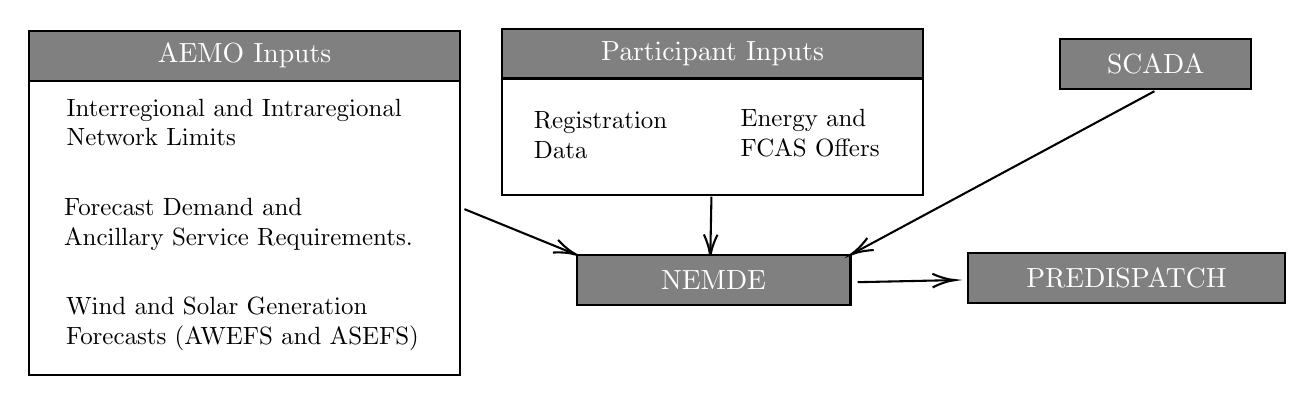
\begin{tikzpicture}[x=0.75pt,y=0.75pt,yscale=-1,xscale=1]
%uncomment if require: \path (0,191.0132598876953); %set diagram left start at 0, and has height of 191.0132598876953

%Straight Lines [id:da9177958313522097] 
\draw    (357.44,91.83) -- (356.91,119.02) ;
\draw [shift={(356.87,121.02)}, rotate = 271.13] [color={rgb, 255:red, 0; green, 0; blue, 0 }  ][line width=0.75]    (10.93,-3.29) .. controls (6.95,-1.4) and (3.31,-0.3) .. (0,0) .. controls (3.31,0.3) and (6.95,1.4) .. (10.93,3.29)   ;

%Straight Lines [id:da12798518797085823] 
\draw    (238.44,97.83) -- (290.59,119.07) ;
\draw [shift={(292.44,119.83)}, rotate = 202.17000000000002] [color={rgb, 255:red, 0; green, 0; blue, 0 }  ][line width=0.75]    (10.93,-3.29) .. controls (6.95,-1.4) and (3.31,-0.3) .. (0,0) .. controls (3.31,0.3) and (6.95,1.4) .. (10.93,3.29)   ;

%Shape: Rectangle [id:dp13477801690658042] 
\draw   (256.5,10.9) -- (459.5,10.9) -- (459.5,90.9) -- (256.5,90.9) -- cycle ;
%Shape: Rectangle [id:dp8582430372753662] 
\draw  [fill={rgb, 255:red, 128; green, 128; blue, 128 }  ,fill opacity=1 ] (256.5,10.9) -- (459.5,10.9) -- (459.5,34.9) -- (256.5,34.9) -- cycle ;
%Shape: Rectangle [id:dp5655505133083187] 
\draw   (28.5,11.9) -- (236.44,11.9) -- (236.44,177.9) -- (28.5,177.9) -- cycle ;
%Shape: Rectangle [id:dp5185219575052318] 
\draw  [fill={rgb, 255:red, 128; green, 128; blue, 128 }  ,fill opacity=1 ] (28.5,11.9) -- (236.44,11.9) -- (236.44,35.9) -- (28.5,35.9) -- cycle ;


%Shape: Rectangle [id:dp11057728244309994] 
\draw  [fill={rgb, 255:red, 128; green, 128; blue, 128 }  ,fill opacity=1 ] (292.44,119.83) -- (424.44,119.83) -- (424.44,143.83) -- (292.44,143.83) -- cycle ;
%Shape: Rectangle [id:dp07113446577922766] 
\draw  [fill={rgb, 255:red, 128; green, 128; blue, 128 }  ,fill opacity=1 ] (525.5,15.9) -- (617.44,15.9) -- (617.44,39.9) -- (525.5,39.9) -- cycle ;

%Straight Lines [id:da9707191163095252] 
\draw    (570.87,41.02) -- (426.2,118.88) ;
\draw [shift={(424.44,119.83)}, rotate = 331.71000000000004] [color={rgb, 255:red, 0; green, 0; blue, 0 }  ][line width=0.75]    (10.93,-3.29) .. controls (6.95,-1.4) and (3.31,-0.3) .. (0,0) .. controls (3.31,0.3) and (6.95,1.4) .. (10.93,3.29)   ;

%Shape: Rectangle [id:dp46501665361769806] 
\draw  [fill={rgb, 255:red, 128; green, 128; blue, 128 }  ,fill opacity=1 ] (480.87,118.83) -- (633.87,118.83) -- (633.87,142.83) -- (480.87,142.83) -- cycle ;
%Straight Lines [id:da4584246014213331] 
\draw    (427.87,133.02) -- (472.87,132.06) ;
\draw [shift={(474.87,132.02)}, rotate = 538.78] [color={rgb, 255:red, 0; green, 0; blue, 0 }  ][line width=0.75]    (10.93,-3.29) .. controls (6.95,-1.4) and (3.31,-0.3) .. (0,0) .. controls (3.31,0.3) and (6.95,1.4) .. (10.93,3.29)   ;


% Text Node
\draw (358,22.9) node [color={rgb, 255:red, 255; green, 255; blue, 255 }  ,opacity=1 ] [align=left] {Participant Inputs};
% Text Node
\draw (304,62) node [scale=0.9] [align=left] {Registration\\Data};
% Text Node
\draw (405,61) node [scale=0.9] [align=left] {Energy and\\FCAS Offers};
% Text Node
\draw (132.47,23.9) node [color={rgb, 255:red, 255; green, 255; blue, 255 }  ,opacity=1 ] [align=left] {AEMO Inputs};
% Text Node
\draw (129.53,105) node [scale=0.9] [align=left] {Forecast Demand and \\Ancillary Service Requirements.};
% Text Node
\draw (127.5,56) node [scale=0.9] [align=left] {Interregional and Intraregional \\Network Limits};
% Text Node
\draw (131.5,153) node [scale=0.9] [align=left] {Wind and Solar Generation \\Forecasts (AWEFS and ASEFS)};
% Text Node
\draw (571.47,27.9) node [color={rgb, 255:red, 255; green, 255; blue, 255 }  ,opacity=1 ] [align=left] {SCADA};
% Text Node
\draw (358.44,131.83) node [color={rgb, 255:red, 255; green, 255; blue, 255 }  ,opacity=1 ] [align=left] {NEMDE};
% Text Node
\draw (557.37,130.83) node [color={rgb, 255:red, 255; green, 255; blue, 255 }  ,opacity=1 ] [align=left] {PREDISPATCH};


\end{tikzpicture}

\caption{AEMO Pre-dispatch Process.}
\label{diagram:predispatch_process}
\end{figure}
\begin{figure}[]
\centering
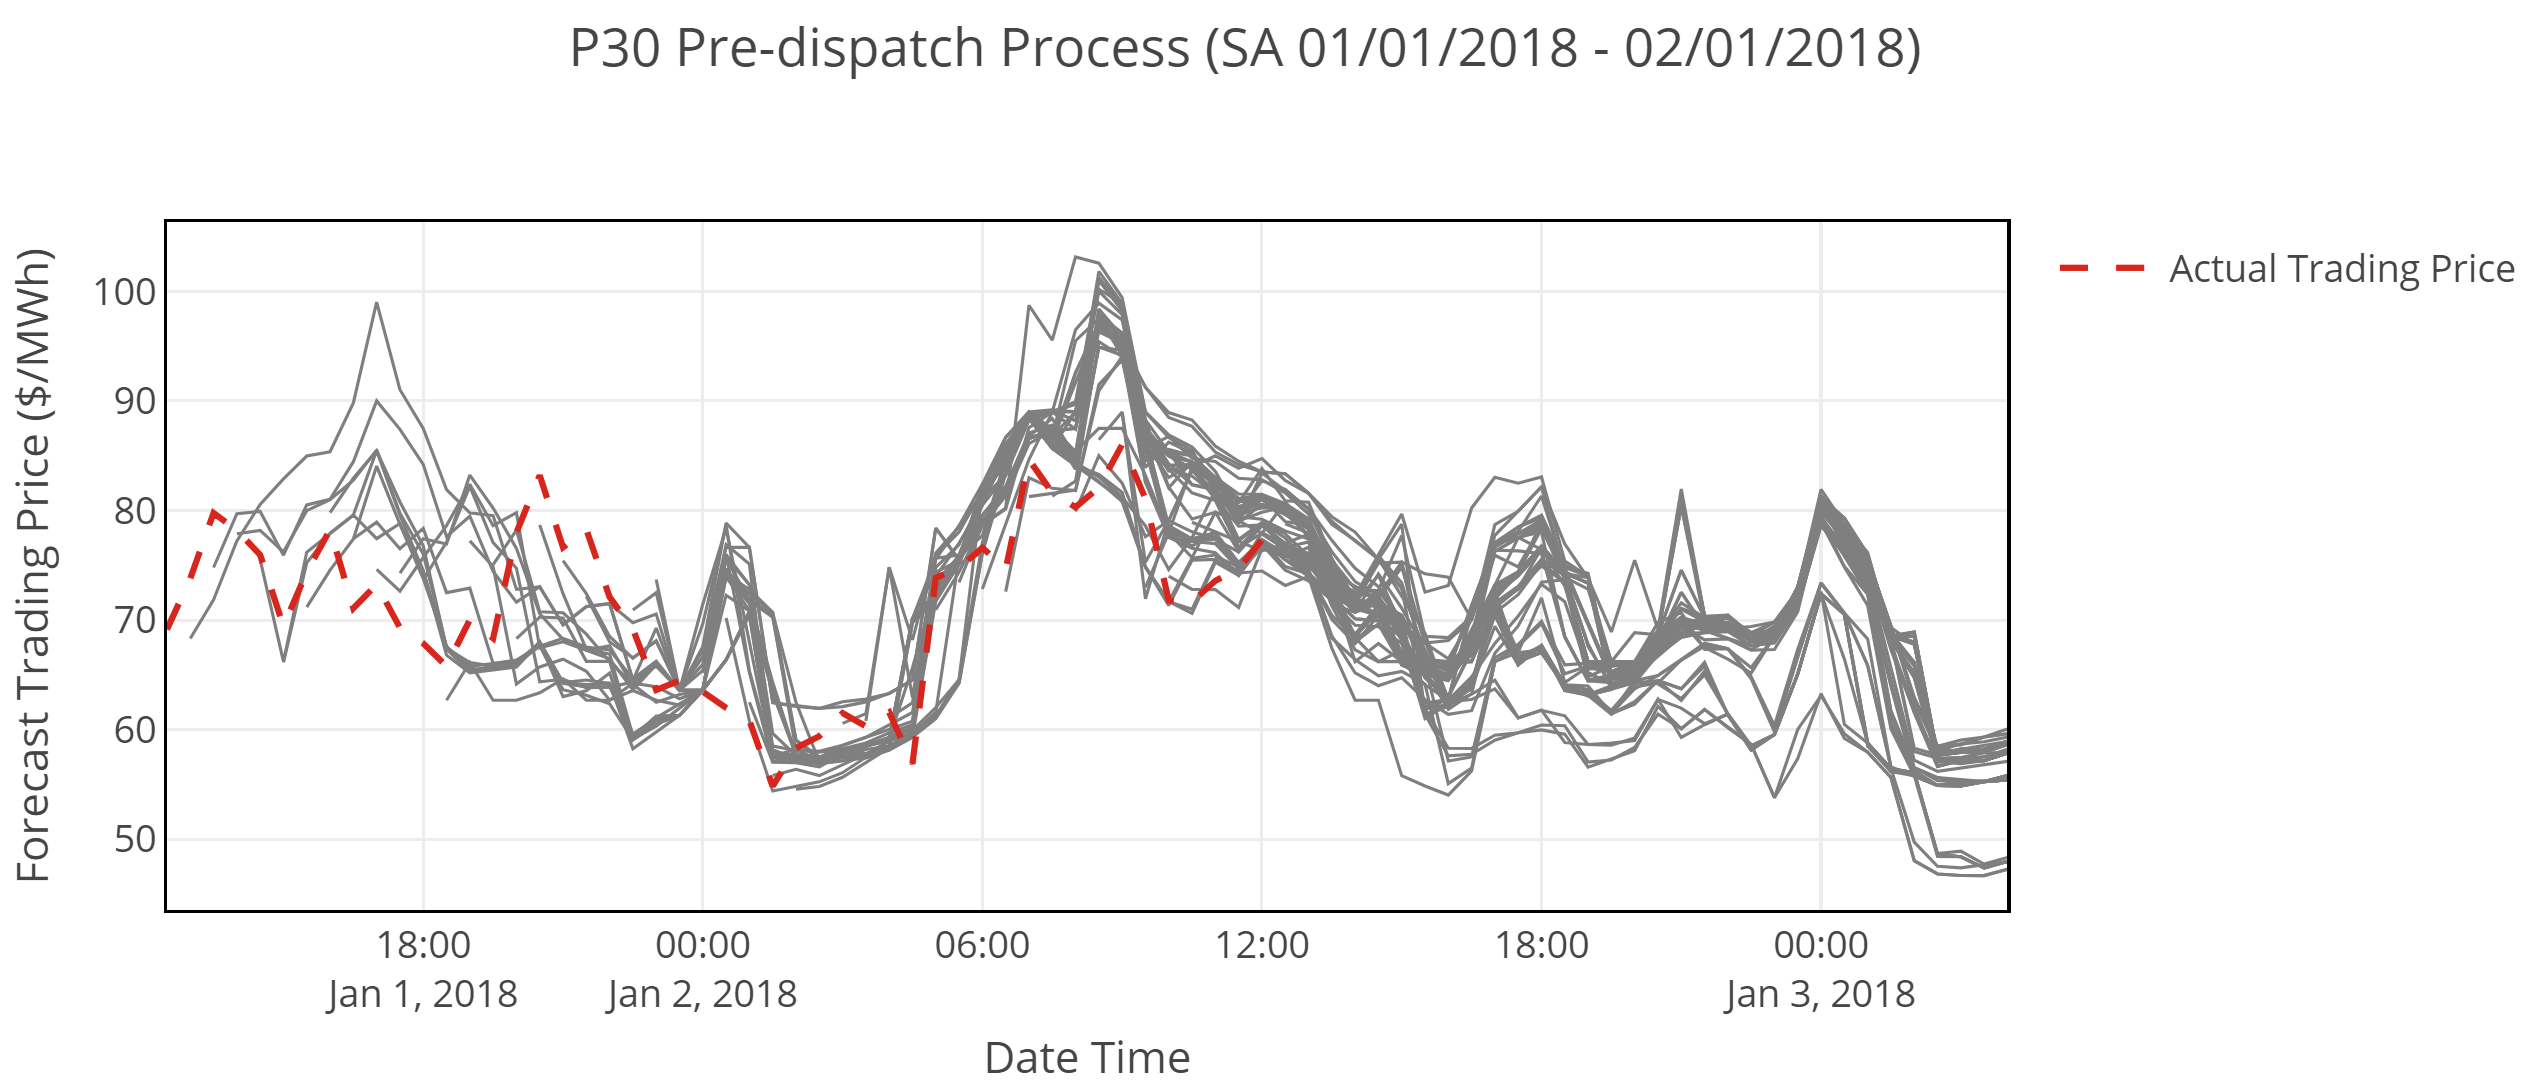
\includegraphics[width=1\textwidth]{Pictures/Chapter2/P30_Process_2.png}
\caption{P30 Pre-dispatch Process - South Australia, 01/01/2018 - 02/01/2018}
\label{fig:p30_process_2}
\end{figure}
Pre-dispatch pricing does vary materially from actual pricing. \textcite{AEMCMarch2017} quantitatively highlighted how predispatch accuracy increases as the dispatch period nears, as shown in Table \ref{table:prediction_aemc}. Table \ref{table:prediction_aemc} highlights also that Tasmania is the worst at predicting high prices. This is likely to be attributable to the fact it is solely owned by Hydro Tasmania with rebidding affecting 65\% of the price spike costs in the state \parencite{AEMCTas}. It is also important to note, NSW and QLD exhibit relatively higher forecast accuracy than the other mainland states.
\begin{centering}
\begin{table}[!h]
\begin{tabular}{l|c|c|c|}
\cline{2-4}
                                   & \multicolumn{3}{l|}{\cellcolor[HTML]{EFEFEF}\textbf{Percentage of Accurately Predicted High Prices}}                                    \\ \cline{2-4} 
                                   & \multicolumn{1}{l|}{\textit{One hour out}} & \multicolumn{1}{l|}{\textit{Four hours out}} & \multicolumn{1}{l|}{\textit{Ten hours out}} \\ \hline
\multicolumn{1}{|l|}{\textbf{NSW}} & 77\%                                       & 66\%                                         & 59\%                                        \\ \hline
\multicolumn{1}{|l|}{\textbf{QLD}} & 73\%                                       & 61\%                                         & 54\%                                        \\ \hline
\multicolumn{1}{|l|}{\textbf{SA}}  & 61\%                                       & 46\%                                         & 39\%                                        \\ \hline
\multicolumn{1}{|l|}{\textbf{TAS}} & 47\%                                       & 38\%                                         & 33\%                                        \\ \hline
\multicolumn{1}{|l|}{\textbf{VIC}} & 52\%                                       & 52\%                                         & 45\%                                         \\ \hline
\end{tabular}
\caption{AEMO P30 Accuracy in Predicting High Prices: 1 September 2015 to 8 March 2017}
\label{table:prediction_aemc}
\end{table}
\end{centering}
\subsubsection{Predispatch Sensitivities}
\label{sec:background_predispatch_sensitivites}
In  addition  to  the  pre-dispatch  prices  run  by  AEMO,  predispatch  price  sensitivities are another data-set published by AEMO. Pre-dispatch sensitivities – also known as  pre-dispatch  scenarios  –  provide  information  on  the  potential  changes  to P30 forecast  regional  spot  prices  and  interconnector  flows  between  regions  as  a  result  of applying pre-defined offsets to the regional demand forecasts used in the base case of pre-dispatch. There are 43 different predispatch scenarios which are explored by AEMO, typically adjusting each NEM region with 8-10 regional demand off-sets. 
\section{ Utility Battery Energy Storage Valuation Models }
\textcite{AECOM} argues utility scale battery storage can provide a wide range of services that yield technical, commercial and economic value. These services can be categorised into four high level functions, as shown in \ref{fig:bess_services}. 
\begin{figure}[H]
    \centering
    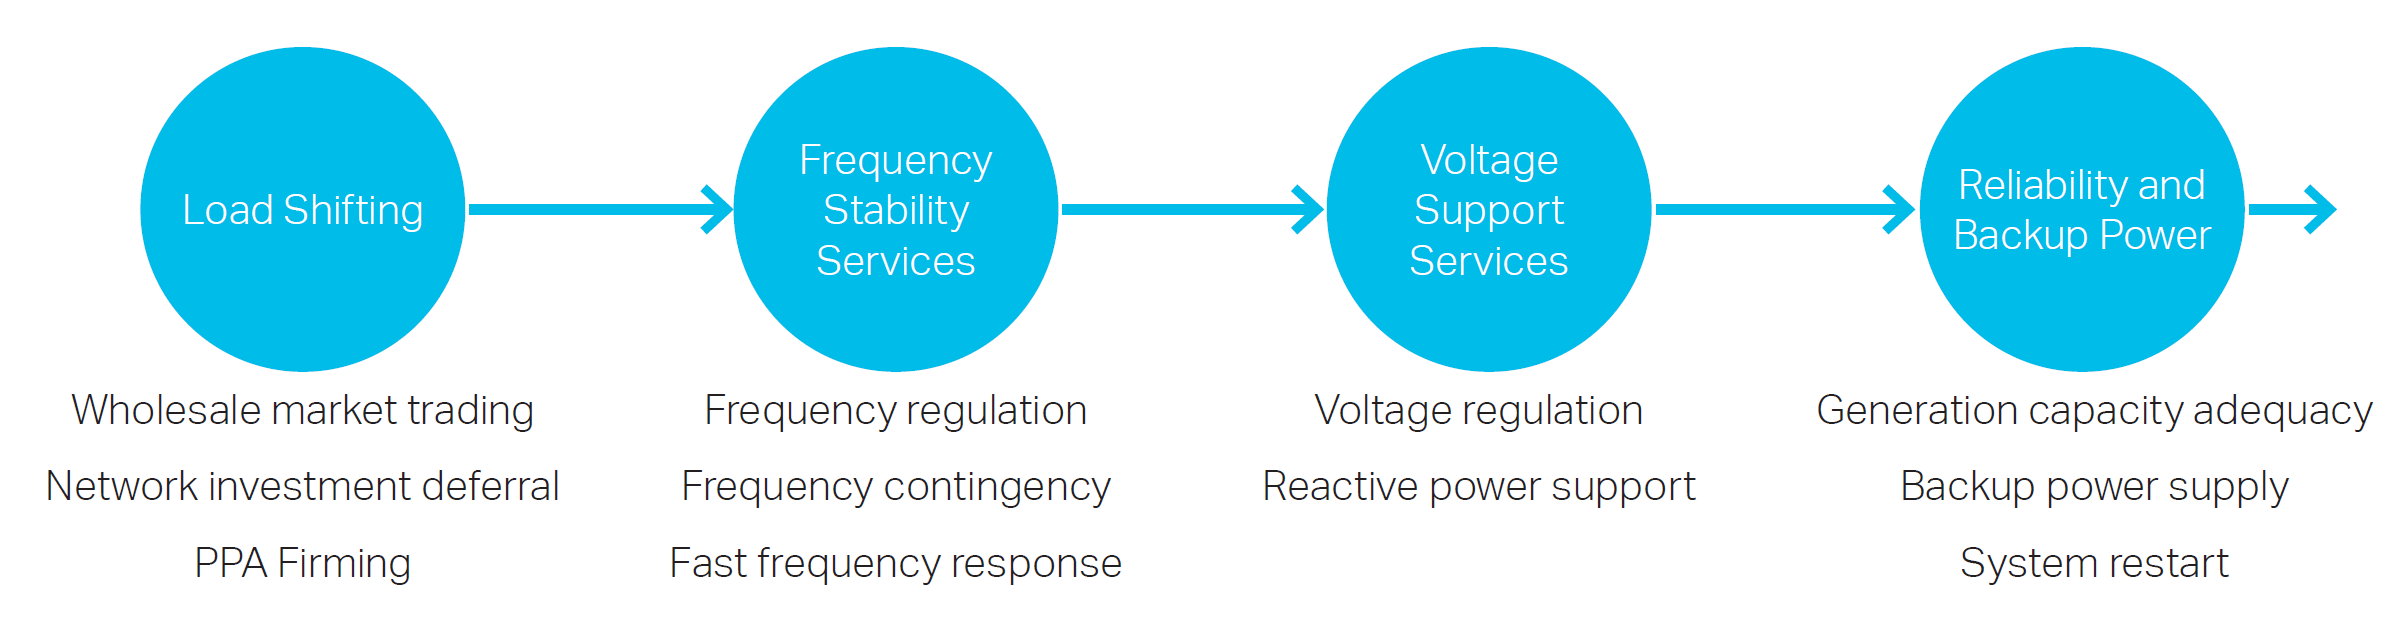
\includegraphics[width=\textwidth]{Pictures/Chapter2/bess_services.png}
    \caption{Overview of utility battery energy services, \parencite{AECOM}}
    \label{fig:bess_services}
\end{figure}
`Load Shifting' via energy arbitrage typically represents the base of the revenue stack offered by utility storage, but generally isn't sufficient to underpin a project financing \parencite{Mackenzie:2018}. Load shifting can also provide physical firming for intermittent generation PPA, or mitigating behind-the-meter curtailment.  Despite the value of PPA firming and curtailment mitigation, quantifying this value stream is highly specific to existing portfolios and contracts of intermittent generation assets. As such PPA firming and curtailment mitigation are not further discussed as they require bespoke valuation and are computationally intractable to co-optimise with other battery functions. 

\subsection{ Energy Arbitrage }
\label{sec:background_energyarb}
 Fundamentally this represents buying wholesale energy on the spot market, storing it in the battery and selling when the price is high. Historically the economic viability of energy storage has been limited to assessing energy arbitrage only, capturing the price differential from electricity spot price volatility. This is value is evaluated using a price-taker model \footnote{A price taker is a person or company that has no control to dictate prices for a good or service.}, or otherwise known as a `small device' energy arbitrage model. In 2008, Sioshansi et al. analysed the PJM interconnection (Sioshansi, 2008). To estimate the arbitrage value of energy storage in PJM from 2002 to 2007, Sioshansi formulated the optimal dispatch profile for a price-taker, energy storage device as a linear problem. In mathematics, linear problems are represented by the form: 
\begin{equation}
    a_1 x_1 + ... a_n x_n + b = 0
\end{equation}
Where ${\displaystyle x_{1},\ldots ,x_{n}}$ are the variables (or unknowns or indeterminate), and ${\displaystyle b, a_{1},\ldots ,a_{n}}$ are the coefficients. Sioshansi defined the energy arbitrage problem via the following parameters. 
\begin{itemize}
    \item \textit{T}: number of hours in a dispatch horizon
    \item \textit{$p_t$}: energy price at hour $t$ 
    \item $\kappa$: power capacity of storage device
    \item $\eta$: round-trip efficiency of the storage device 
\end{itemize}
Additionally decision variables were defined which were calculated at each time step. These included: 
\begin{itemize}
    \item $c_t$: energy charged into the storage device at time $t$
    \item $d_t$: energy discharged from the storage device in hour $t$
    \item $s_t$: energy stored in storage device at the end of hour $t$
\end{itemize}
The problem is formulated as maximizing arbitrage value:
\begin{equation}
    max \sum_{T}^{t=1}p_t \times (d_t - c_t)
\end{equation}
Subject to the linear temporal constraints ($\forall \quad t = 1,2 \dots, T)$: 
\begin{itemize}
    \item storage level: $s_t = s_{t-1} + \eta \times c_t - d_t $
    \item power capacity of the device: $d_t, c_t \in [0, \kappa]$
    \item energy capacity of the device: $s_t \in [0, h \times \kappa]$
\end{itemize}
Sioshansi performed this optimisation over 2 week batches, and used a Linear Programming problem solver CLPEX to efficiently solve this linear problem. Figure \ref{fig:sioshansidispatch} shows the output of this simulation during a given week in 2006, using an 80\% round-trip efficiency.
\begin{figure}[H]
    \begin{center}
        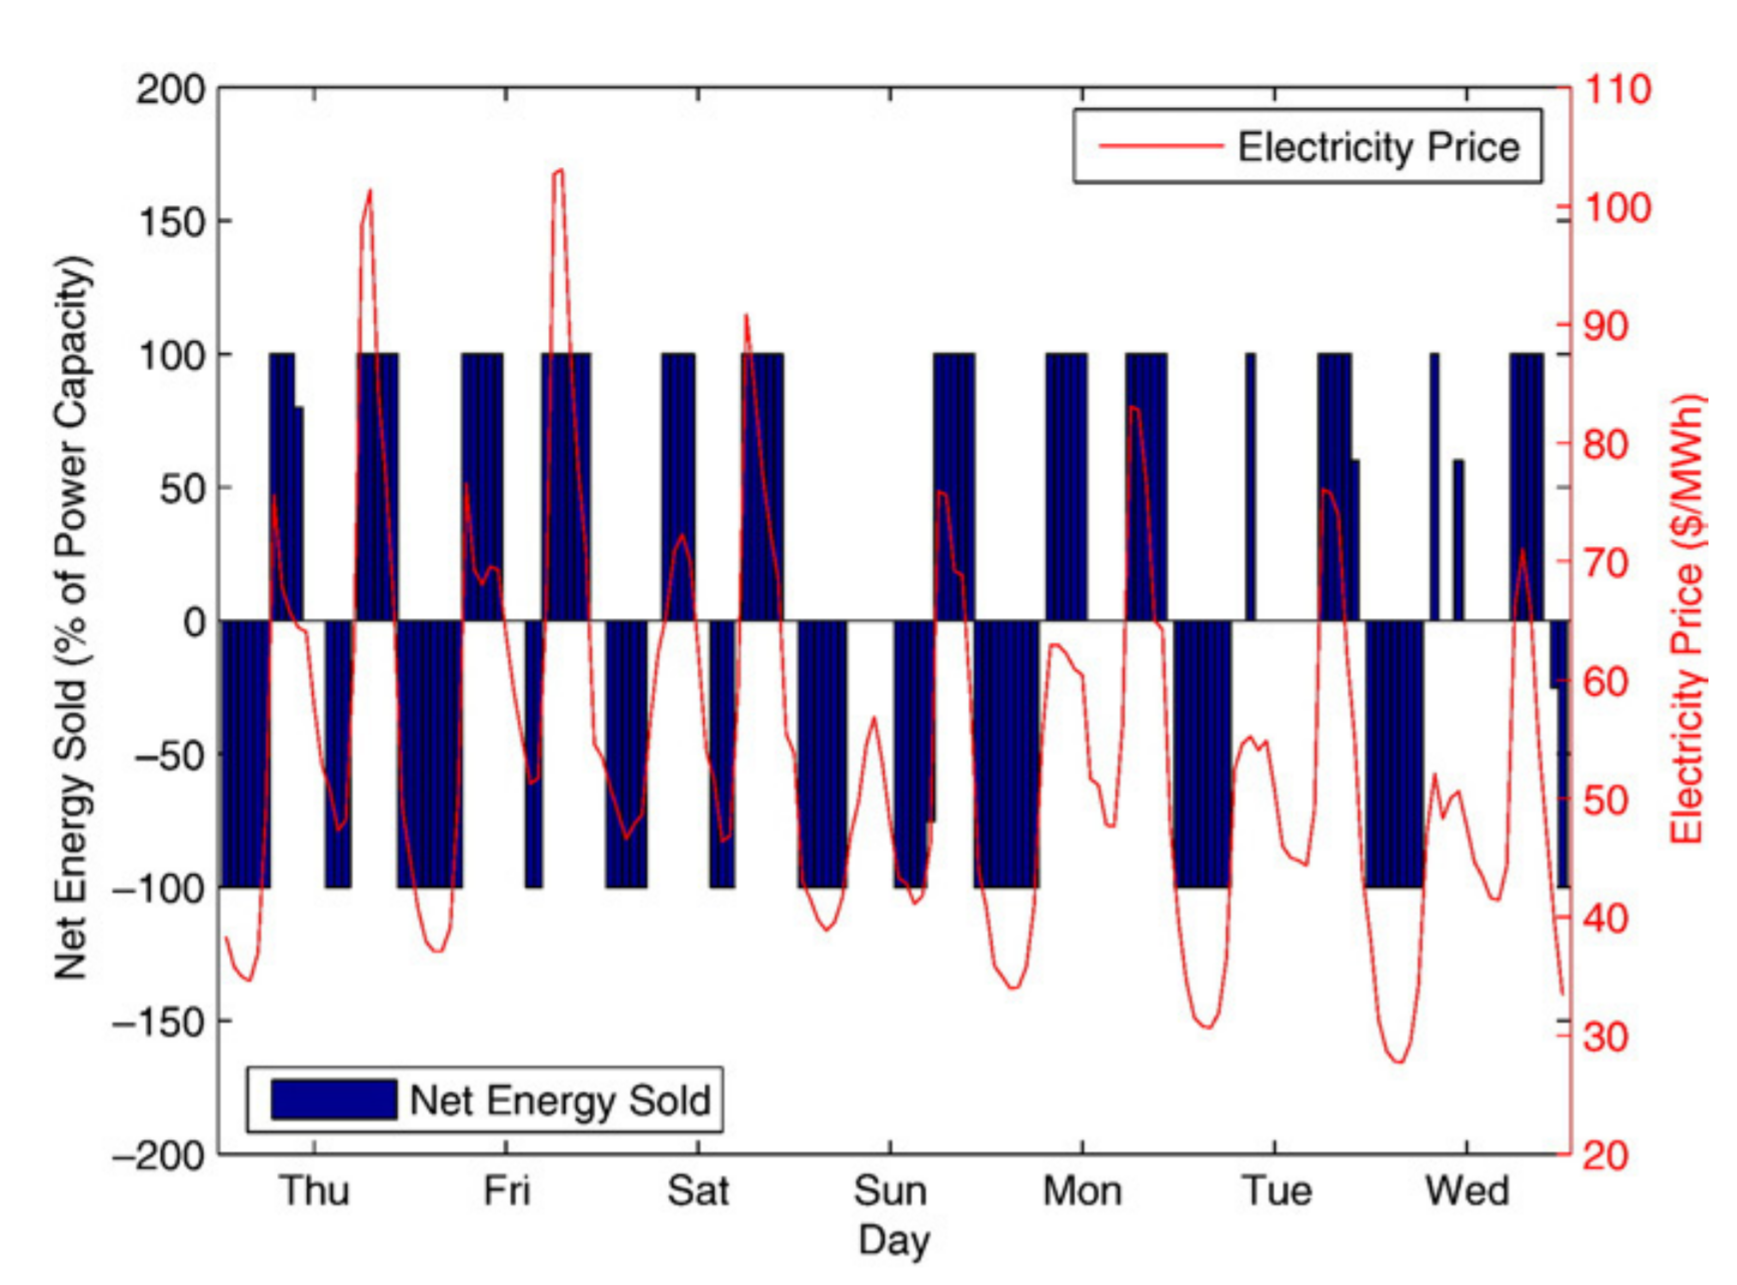
\includegraphics[width=0.6\textwidth]{Pictures/Chapter2/Sioshansi_output.png}
    \end{center}
    
    \caption{Electricity prices and the optimal hourly dispatch of storage device during one
week in 2006 (Sioshansi, 2008) }
    \label{fig:sioshansidispatch}
\end{figure}
The key findings of Sioshansi's research were;
\begin{enumerate}
    \item The marginal arbitrage value (on a \$/kW bases) drops shapely as a function of energy capacity, with the 'knee' of the curve at 8 hours of storage. In other words, rapidly diminishing returns occur for batteries greater than 8 hours of storage. 
    \item The value of energy storage via arbitrage for a 12 hr storage battery was \$110/kW-year.
    \item In practice capturing value through energy arbitrage requires short-term forecasting of price. Using a back-casting approach to predict price instead of perfect foresight, Sioshansi claims the battery only captures 85\% of energy arbitrage revenue. 
\end{enumerate}
In 2014, Sioshansi's work was extended to the Australian NEM context by Wang, Macgill and Bruce. \citep{Wang} analysed the energy arbitrage value of battery energy storage across all NEM regions from 2010-2013. Wang found South Australia was consistently the high performer among NEM regions. Conversely, on average NSW was the worst performer. Wang discovered a heavy dependency of arbitrage value on high price events, demonstrated in NSW where 50\% of the revenue was earned over one day. 
\subsubsection{PJM Example}
More recently \parencite{SallesPJM} assessed the potential value of energy storage in PJM, assuming a price-taker with perfect foresight in the real-time market. PJM provides participants with the option to participate in a day-ahead market or in a real-time balancing market. The real-time market is dispatch every 5 minutes but actual financial settlement occurs hourly. PJM also employs locational marginal price (LMP) which is defined as the price of supplying an additional MW of
load at a specific location in the power system. Similar to McConnell and Wang, Salles employed Linear Programming. Salles emphasised the notion of diminishing returns as you increase the energy/storage ratio for a BESS.
\subsection{ Energy Arbitrage with Imperfect Foresight }
One of the limitations of this basic arbitrage analysis is the perfect foresight assumption for energy prices. There is substantial uncertainty around short-term future electricity prices, particularly in the case of scarcity events and extreme price spikes in an energy-only market \parencite{McConnell}. 
Sioshansi et al. used a back-casting approach in order to forecast price and produce a dispatch schedule based on historic prices for the previous two weeks. Sioshansi finds the back-casting approach provides 85\% of the optimal perfect foresight revenue, however given the fact PJM has entirely different market design this benchmark provides little insight for NEM-based battery energy storage systems. 

\parencite{Wang} analysed the impact of imperfect foresight on battery revenue for 2010, and 2013 in the NEM using a rolling window of P30 price-forecast to inform battery dispatch. Wang found that for a 1MW, 1MWh battery imperfect foresight captures approximately 30\% of optimal revenue for mainland states. Wang also discovered that increasing the hours of storage up to 8 hours (8MWh) can increase the percentage of revenue under imperfect foresight of price up to approx. 60\% in VIC and SA and approx. 50\% in NSW and QLD.
2
\parencite{McConnell} similarly explores the impact of imperfect foresight on battery energy arbitrage revenue claiming increasing the storage improves the realisation of potential arbitrage value, from 70\% at 3 h to over 90\% at 8 h, using FY 13-14 price data for South Australia, shown below in \ref{fig:mcconnel_2014}. This is a similar trend to Wang highlighting that as storage increases the percentage of optimal revenue which can be captured also increases. McConnell describes that this may be due to increased flexibility of the storage device i.e. The ability to re-evaluate and change operation may be constrained for smaller device. 
\begin{figure}[H]
    \centering
    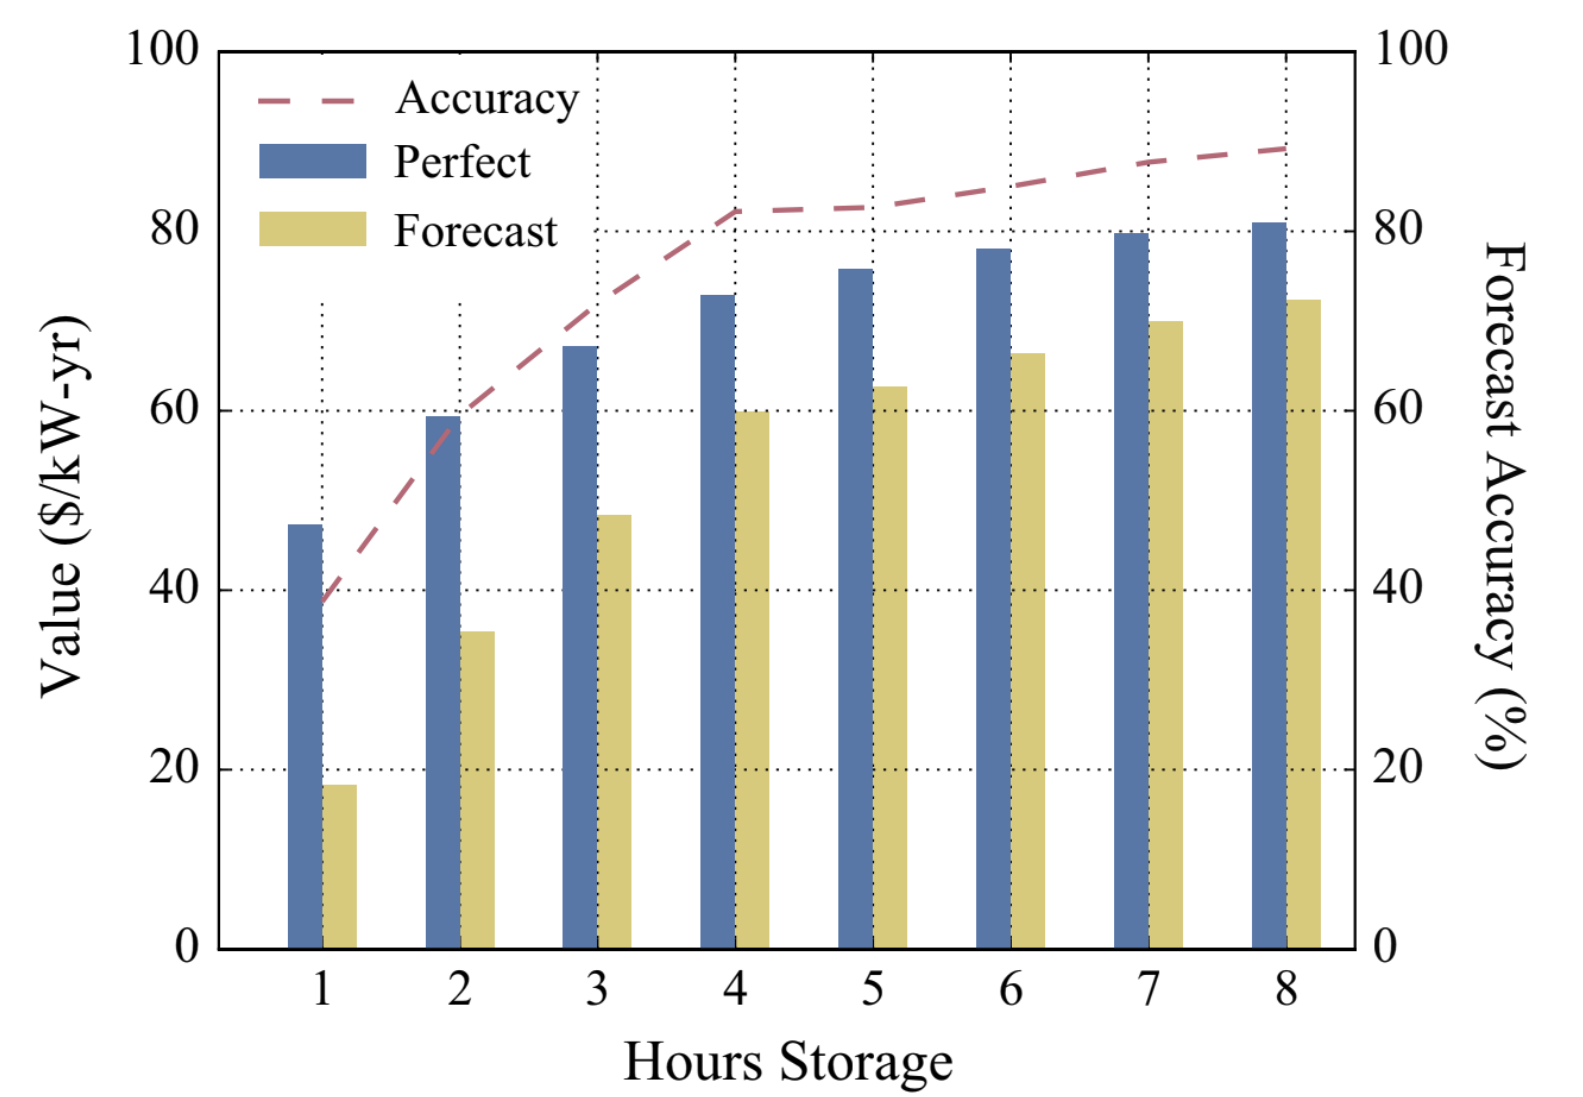
\includegraphics[width=0.5\textwidth]{Pictures/Chapter2/mcconnel.png}\
    \caption{Forecast vs perfect foresight for FY 2013–14. Value comparison (\$/kW-yr,
left hand axis) and accuracy (\%, right hand axis). Source \parencite{McConnell}}
    \label{fig:mcconnel_2014}
\end{figure}
\subsection{ Energy Arbitrage with Co-optimised with FCAS Participation }
\label{cooptimisation}
Recapping Section \ref{fcas} in the NEM frequency control ancillary services (FCAS) are required to maintain the frequency of the power system within the frequency operating standards. There are two general categories of FCAS; \textbf{regulation services}, which continuously adjust to small changes in demand or supply, and \textbf{contingency services}, which manage large changes in demand or supply that occur relatively rarely and move the frequency by a large amount.
As contingency events occur relatively rarely, co-optimisation in this thesis refers to co-optimising energy and regulation dispatch.

In the NEM, FCAS markets are settled every 5 minutes with the following formula:
\begin{equation}
    \text{Payment} = \text{MWE} \times CP/12 
\end{equation}
Where MWE is the amount of MWs enabled for the FCAS and CP is the clearing price for the service in that dispatch interval. The FCAS markets are to ensure the stability and security of the power system because the demand and supply of electricity have to balance instantaneously. The FCAS participants make capacity reserve offers to AEMO and AEMO determines the amount of capacity reserves required in each FCAS market dynamically according to the rules. The reserve offer represents the amount of power that a FCAS market participant is able to raise or lower within a specified time frame. The FCAS market participants are paid for the reserves offered to AEMO if they are not instructed to alter the power dispatch level. Once the instructions are issued, they are also paid or need to pay for the amount of energy delivered or received at the spot trading price. The FCAS instruction is termed “AGC energy delivered”. The concept of “AGC energy” often misunderstood as participants are paid through the FCAS markets in accordance with their offered volumes. Their energy production, that may be higher or lower depending on the AGC signals they receive, are settled in accordance with energy market prices (Report into market ancillary service prices above \$5000/MW \parencite{AEMO_FCAS_REPORT}.
\newline
\newline
Offers and bids for the FCAS services take the form of the generic FCAS trapezium, shown in Figure \ref{fig:fcas_trapzium}; defined by enablement limits and breakpoints. The trapezium indicates the maximum amount of FCAS that can be provided for a given MW output level for a generator, or given MW consumption level for a scheduled load. 
\begin{figure}[H]
    \centering
    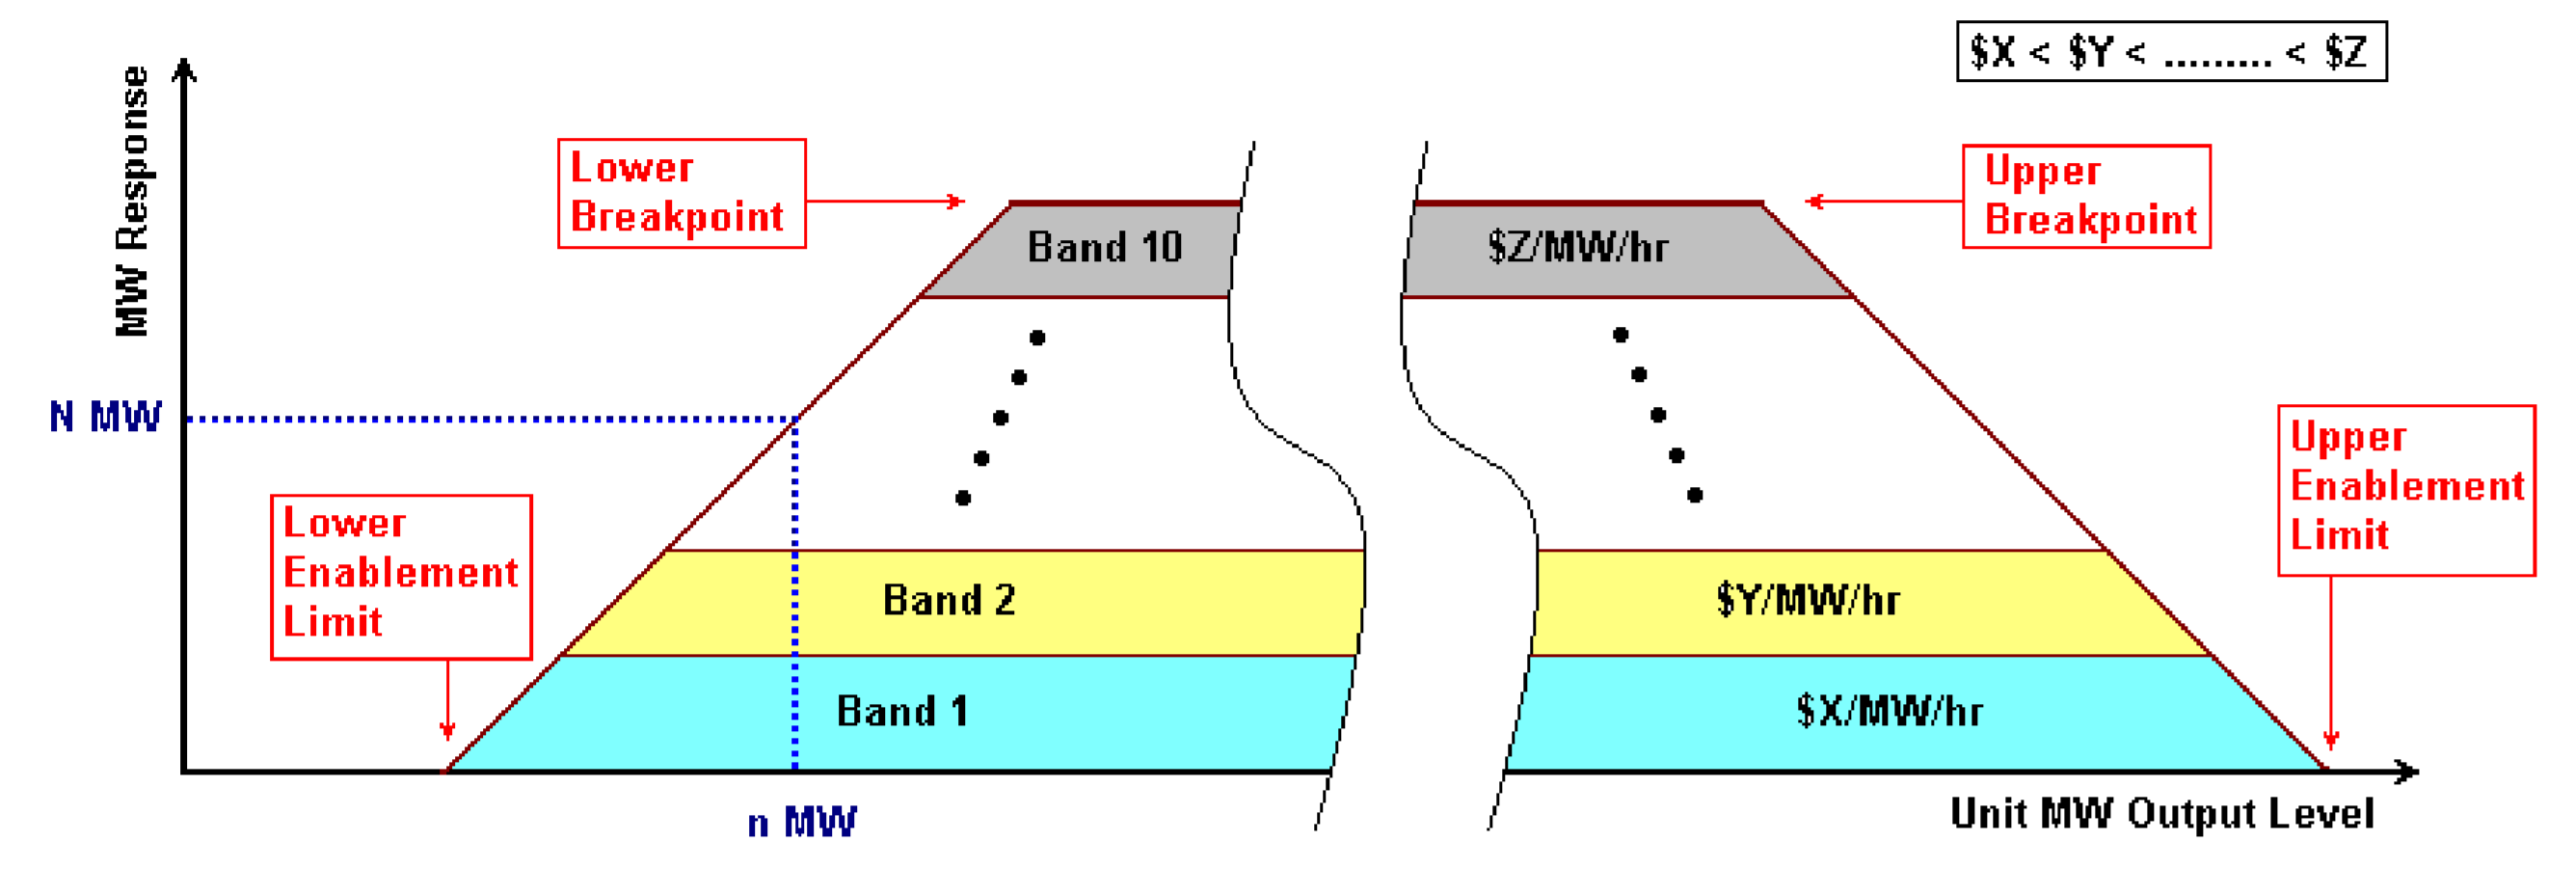
\includegraphics[width=0.8\textwidth]{Pictures/Chapter2/fcas_trap.PNG}
    \caption{ Generic FCAS Trapezium \parencite{AEMO_NEM}}
    \label{fig:fcas_trapzium}
\end{figure}
As shown in Figure \ref{fig:fcas_trapzium}, an enablement on FCAS comes at opportunity cost of energy market enablement. At a maximum energy output no FCAS raise services can be offered, similarly if a battery is entirely empty no regulation services can be provided. Figure \ref{fig:energy_and_reg} shows typical day for energy and regulation prices. The challenge of co-optimisation involves capturing energy arbitrage revenue via a price differential whilst also providing an optimal combination of services in ancillary markets.
\begin{figure}[H]
    \centering
    \makebox[\textwidth][c]{    \includegraphics[width=1.1\textwidth]{"Pictures/Chapter2/Energy and Regulation Prices".pdf}}
    \caption{Energy and Regulation Spot Prices - 2018-01-01}
    \label{fig:energy_and_reg}
\end{figure}
As shown in Figure \ref{fig:energy_and_reg}, regulation prices are typically much lower than bulk energy services. As such an asset solely participating regulation services is unlikely to be profitable. However, as regulation is a standby service there is still a revenue opportunity for a asset participating in energy arbitrage.
\newline
\newline
Existing literature on the co-optimisation of energy arbitrage and regulation services in the NEM is extremely limited and isn't usually performed from a financial evaluation perspective. 
(Kazempour, 2009) addressed this problem from the context of pumped hydro maximising profit via hourly production bids in the energy and the regulation markets. Kazempour assumes perfect foresight and price-taker assumption, and employs non-linear mixed integer programming (NLMIP) to solve the problem. 
\newline 
\newline 
\parencite{Donadee} explored the co-optimisation of the operations of a grid scale energy storage resource for both energy price arbitrage and secondary frequency regulation capacity. Unlike (Kazempour, 2009), Donadee does not assume perfect foresight of energy prices an consequentially used an infinite horizon Markov Decision Process  (MDP) in order to optimise a BESS with 50MWh and 15MW.  The ESR SOC was discretized with 11, giving 264 possible states. Donadee used real-time energy market prices from PJM on 2010-01-08. Donadee also only employed a static price for regulation capacity. The first case assumed a constant regulation capacity price of \$0/MW. In the second and third cases he assumed constant regulation capacity prices of \$20/MW and \$60/MW. Donadee found when the regulation price is \$60/MW, the total revenue is more than double that of the \$0/MW case. 
\newline
\newline
\parencite{Zhai:2018} presents the only body of work which to date has extended co-optimisation across energy and regulation markets to a NEM context. Zhai used historical prices from South Australia from May 1st to May 31st 2014. \parencite{Zhai:2018} employed a modified dynamic programming algorithm with perfect foresight of price to dispatch the battery across energy and regulation markets. In order to determine the AGC energy component each interval, Zhai discovered hourly correlations AGC energy. Zhai found that the BESS makes 2 times more revenue when participating in regulation and energy markets. 

\subsection{ Performance of Existing Utility Battery Energy Storage Plants in the NEM }
\subsubsection{ Hornsdale Power Reserve }
\label{hornsdale}
On December 1st 2017 Neoen deployed the Hornsdale Power Reserve, also known as the ``Tesla Big Battery". According to \parencite{HornsdaleRenewEconomy}, the cost of the battery was \$90m AUD. At 100MW/129MWh, the Hornsdale Power Reserve is the largest lithium-ion battery in the world \parencite{HornsdaleWebsite}. The HPR provides a range of services under commercial agreements between the South Australian Government, Tesla (the battery technology provider), and NEOEN (the operator). The services are summarised below provided from AEMO's report: Initial Operation of Hornsdale Power Reserve Battery Energy Storage System \parencite{HornsdaleReport}:
\begin{itemize}
    \item \textbf{Energy Arbitrage:} Under normal conditions, 30 MW of the battery’s discharge capacity is made available to Neoen for commercial operation in the National Electricity Market (NEM). Of the battery’s total 129 MWh energy storage capacity, 119 MWh may be used for this mode of operation.
    \item \textbf{Reserve Energy Strategy:} The remaining 70 MW of battery discharge capacity is reserved for power system reliability purposes.
    \item \textbf{Network loading control ancillary services (NLCAS):} The HPR is included in a new control scheme – the System Integrity Protection Scheme (SIPS) – which is intended to reduce the likelihood of the South Australia power system separating from the rest of the NEM following a sudden increase in flow on the Heywood Interconnector. \parencite{HornsdaleRenewEconomy} also announced that the contract with the South Australian Government is \$4 million for this contract. 
    \item \textbf{Ancillary Services (FCAS):} The HPR is registered to provide all eight FCAS services, and actively participates in all eight FCAS markets.
\end{itemize}
According to \textit{RenewEconomy} the Hornsdale Power Reserve has made \$2.5 million  in 3 months from January 1 to March 31, as seen in Figure \ref{fig:hpr_3_mon_rev}. The biggest contributor came from energy arbitrage. AEMO estimates that half of this \$2.3 million of revenue was generated across three days in January and February, when prices surged to or near the market cap. It also earned money from FCAS regulation and contingency markets, and according to AEMO was active in FCAS markets 99.5\% of the time. Furthermore, \textcite{HornsdaleRenewEconomy} highlighted that the average charge price during this time was \$70/MWh and average discharge price \$170/MWh. 
\begin{figure}
    \centering
    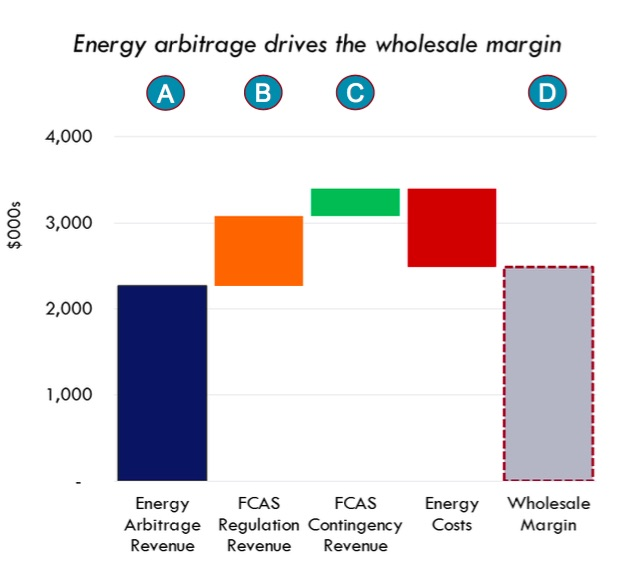
\includegraphics[width=.6\textwidth]{Pictures/Chapter2/hpr_first_3_months.jpg}
    \caption{Hornsdale Power Reserve Revenue: January 1 to March 31, 2018}
    \label{fig:hpr_3_mon_rev}
\end{figure}
After 12 months of operation, Dylan McConnell from the Melbourne Energy Institute estimated the annual revenue of the entire 90MW / 129MWh battery, shown in Figure \ref{fig:hpr_12_mon_rev}. In Figure \ref{fig:hpr_12_mon_rev}, the contingency revenue is substantially large due to the enablement of the full 100MW bid into the contingency markets. 
\begin{figure}
    \centering
    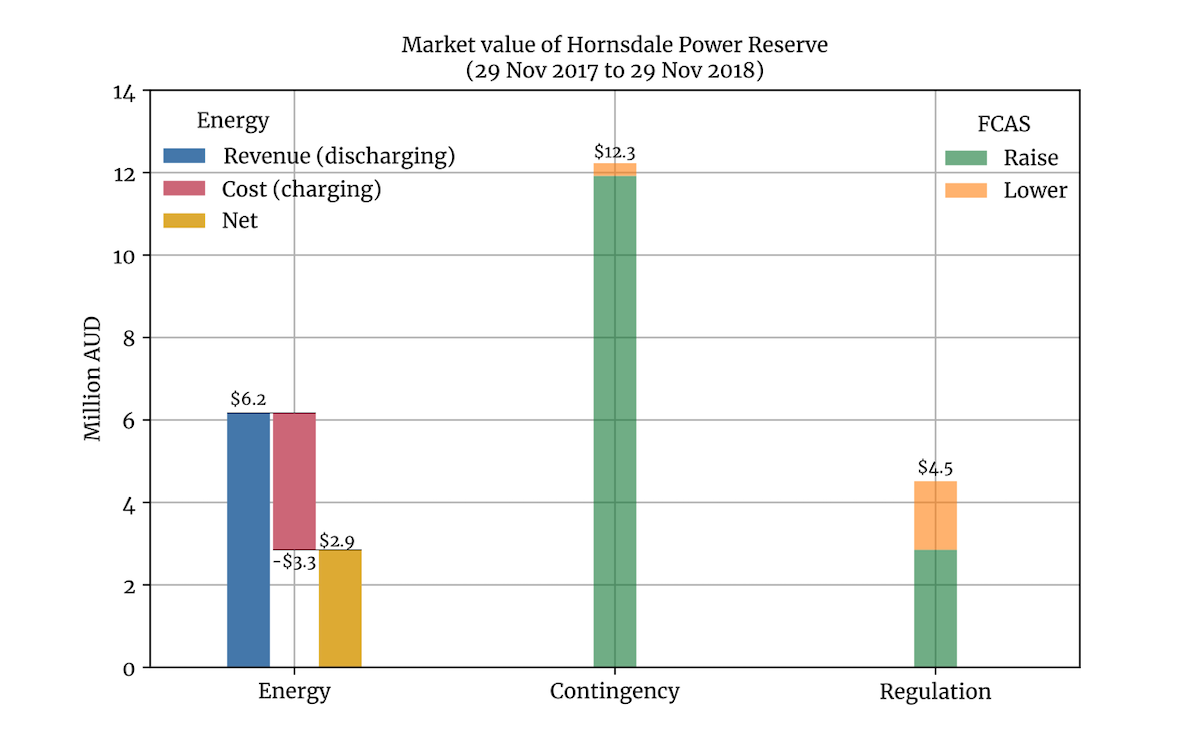
\includegraphics[width=.8\textwidth]{Pictures/Chapter2/hpr_revenue.png}
    \caption{Hornsdale Power Reserve: 29 Nov 2017 - 29 Nov 2018}
    \label{fig:hpr_12_mon_rev}
\end{figure}
\parencite{hornsdale_savings} highlights netted \$2.86 million of net revenue from energy market trading, in addition to another \$16.75 million from FCAS market. Furthermore, Hornsdale's \$4 million contract with the Australian Government for grid security services, totals \$24 in revenue in the first year. 
\subsubsection{ Lake Bonney Battery Energy Storage System }
\label{sec:ifn}
On August 15th 2018, Infigen Energy (ASX:IFN), announced investment in a 25 MW / 52 MWh battery sotrage system adjacent to their existing 278.5 MW Lake Bonney Wind Farm \parencite{IFN_AFR}. \textcite{IFN_AFR} also highlights the BESS cost \$38 million with \$10 million in state and federal funding. The BESS is expected to be participating the market in Q3 2019.
